
\chapter{Hash Table\index{Hash table}}\label{Hash table}

In this chapter, we will return to the primitive components of our data structure that are hash tables\index{Hash table}. We will come back to the different possible implementations and will try to compare them in the concurrent\index{Concurrent} framework. This will allow us to define a hash table\index{Hash table} that can be used as a base block in our X-fast trie\index{X-fast trie} to test parallelism capabilities for our data structure. We will focus mainly on insertion and search capabilities based on a single thread since this kind of operations will be the most useful to us.

\section{General context}

Hash tables\index{Hash table} play an important role in many algorithms and data structures. It is a fundamental data structure which can be used at many places. They can be seen as a bunch of slots where elements will be stored and every possible item from the universe will be mapped to one of the slots thanks to a hash function. Nevertheless, there can be collisions since the number of available slots is very much smaller than the size of the universe and thus each location can have multiple items mapped to them. Classical techniques of collision resolution must be adapted to GPUs\index{Graphics cards} due to their nature highly parallel:

\begin{itemize}
    \item Serialization: of the operations, indeed we cannot use locking mechanism on GPU\index{Graphics cards} and we must thus find solution without those and with the help of atomic\index{Atomic} operations. Those algorithms and data structures are often qualified as \textit{lock-free} if it guarantees system-wide progress or \textit{wait-free} if it also per-thread progress.
    \item Memory accesses: threads are intended to be used together to benefit from coalesced memory but the inherent nature of hash table\index{Hash table} makes it hard since the elements are randomly spread.
    \item Probing\index{Probing}: another big aspect is the warp notion, all the threads will have to wait for the slowest one, hence the worst-case number of probes required.\\
\end{itemize}

This structure is characterized by a memory-intensive task linked to the presence of numerous random accesses and, as GPUs\index{Graphics cards} present a very interesting memory bandwidth, it makes them good candidates for such structures. The goal is then to make the most of the parallelism offered, either through a data parallelism between the threads, or a work as little divergent as possible between all the elements of the same warp. These parallelism elements can also be used to simplify probing\index{Probing} by performing all accesses related to the following probes in one treatment. Finally, it is also interesting to reduce the number of atomic\index{Atomic} operations that are carried out. These induce a not insignificant cost when there are so numerous but they are also the only primitives ensuring the validity of the accesses on GPU\index{Graphics cards}.

There exist several ways to construct those data structures:

\begin{itemize}
    \item Perfect Hashing\index{Perfect hashing}: The best way to handle $O(1)$ operations and not to have troubles with collisions is to avoid collisions thanks to perfect hashing\index{Perfect hashing}. M. L. Fredman, J. Komlós and E. Szemerédi~\cite{fredman1984storing} introduced a simple construction at the price of space efficiency $O(N^{2})$. The problem consists essentially to find a hash function that will not cause collisions. There are $\binom{N}{2}$ pairs who can collide each with probability $N^{2}$, hence there is $\binom{N}{2} / N^{2} < \frac{1}{2}$ chance that there is a potential collision. Otherwise the other idea is to do a perfect hashing\index{Perfect hashing} on $O(N)$ elements and do the same thing on collisions (combining with the chaining\index{Chaining} idea), this allows to make it dynamic~\cite{dietzfelbinger1994dynamic}.
    \item Open Addressing\index{Open addressing}: A simple technique to implement, in order to insert an item, a series of probes is performed until an empty slot is found. There are three common strategies to probe: linear, quadratic and double hashing. Those probes must set the value atomically\index{Atomic} if it the key is empty, care must be taken with deletion. Problems also appear when the load factor is too important and the variance on the queries can be quite large. Resizing the table is also not trivial due to the expected lazy initialization of the new table~\cite{gao2005lock}. The expected number of probes is bounded by $1/(1 - \frac{N}{m})$ due to the hypergeometric probability where $m$ is the number of slots in total.
    \item Chaining\index{Chaining}: An alternative is to use a set of buckets and add elements in a linked-list fashion. But traversing pointers is generally not efficient. This approach can be completed by grouping the elements into larger packets~\cite{ashkiani2017dynamic} but variance can still be high if there are not enough buckets. Nevertheless, the possibilities of lock-free algorithms are numerous and they also guarantee the validity of iterators combined with resource management (garbage collector). The expected work is in $O(1 + \frac{N}{m})$ where $m$ is the number of buckets/chains. On average, for all the insertions, we get: $\frac{1}{N} \sum_{i=0}^{N-1} (1 + \frac{i}{m}) = O(1 + \frac{N}{m})$
    \item Cuckoo\index{Cuckoo hashing}: it ensures a small number of probes by limiting the number of slots an item can reside. The idea is that the elements are exchanged from one table to another each time a collision occurs. However, we may need to reconstruct the table entirely. There are some technical difficulties to implement those but they present fair results~\cite{alcantara2009real}. It is possible to show that if the load factor is less than $\frac{1}{2}$, the expected number of evictions is constant and the longest path is bounded by $O(\log N)$. Beyond, cycles may appear and there are specific solutions to solve those issues.
\end{itemize}


\section{Implementation}

We will come back to some points linked to these data structures which seem for us important. In practice, LSMs\index{LSM} are way easier to implement than X-fast tries\index{X-fast trie}.

\subsection{X-fast trie}

We started by looking to see if there was any work on how to make x-fast tries\index{X-fast trie} concurrent\index{Concurrent} and we did not come across any results in this direction. So we tried to do what we could to solve the problem.

In practice, making the data structure concurrent\index{Concurrent} does not seem to be an impossible task even if it is somewhat difficult and much attention must be paid to it. We started by making ``atomic'' the internal nodes of the tree, i.e. if two threads try to insert the same node into the tree, the second will necessarily apply the procedure of merging (upsert) on the data it was in charge of and the one previously inserted. The merge procedure is the same as the node update procedure, atomically replaced in order to keep the key of the minimum and maximum element of the whole subtree.

Note that node updating plays a very important role in this concurrent\index{Concurrent} problem. Indeed, when one wishes to insert a node at the level of the leaves, one wants to have the smallest interval of values which exists and which contains the key of the new element. This avoids having to go through too many elements and therefore minimises the concurrency\index{Concurrent} problems there, by minimising the time spent there. The first step is to insert the element with its closest neighbors into the data structure. This avoids searching for an element that does not yet exist in the leaves but is described in the intermediate nodes.

Now all that remains is to correct it and update its neighbours to indicate its existence. The same procedure is always followed until the situation is resolved. The aim is to reduce the interval while it is possible. We update the predecessor and successor values of the node we want to insert. We make a ``compare and swap''\index{Compare and swap} on the previous node to put ourselves as successor, idem for the next one, we modify its predecessor. If both succeed, then we're done. Otherwise, the procedure is repeated again. Boundary and degenerate cases are limited by the fact that the structure provides the smallest interval ab initio.

\subsection{LSM\index{LSM}}

We tried to obtain the LSM\index{LSM} source code from the authors, who politely declined our request. We have therefore sought to replicate it based on the description made in their article which is nevertheless sufficiently clear and precise. We used the same two primitives to sort our data and merge dictionaries. And we hope we have provided an implementation that we feel is relatively fair and sufficiently close to what they have done. The structure being very simple, variations on possible implementations should be minor.

One of the key points of this structure is its inherent sequentiality\index{Sequential}. It seems difficult to propose a concurrent\index{Concurrent} version or, at least, to have something effective. We have to wait until the treatment between two levels is completely done before we can do anything else. As there are also very few levels in the structure, a very huge contention will be observed on the first levels making it essentially serialized. It was also easier to use two buffers to merge our data, as suggested in the original paper. So we work on a single block and on only 16 warps out of 32 available. Indeed, the library we use to sort requires some ``shared'' space (linked to a block) that we did not have enough to support 32 warps per block.


\section{Experiments}\label{PARALLELXFASTTRIERESULTS}

For the experiments, we have again put in place a simple experimental protocol. We tested the three canonical operations: insertion, search and predecessor query, the ones that interest us the most, we can expect an equivalent time for successor or deletion requests. We compared the performance obtained for three different data structures, X-fast tries\index{X-fast trie}, B-trees and LSM\index{LSM}; each under special conditions.

For the insertions, the B-trees\index{B-tree} have no concurrent\index{Concurrent} version known as being really effective, we therefore reused the data structure developed in the chapter relating to X-fast tries$^{[\ref{BTREE}]}$ and this in a sequential\index{Sequential} context, i.e. with only one warp in only one block.

For LSM\index{LSM}, the situation is different, first, it is difficult to provide true parallelism to this data structure given its inherent sequentiality\index{Sequential} and, second, for technical reasons, we have not been able to launch more than 16 warps related to too much shared memory use for the sort primitive used.

Finally, for the X-fast tries, the problem was quite different, crashes appeared in some rare case. Of course, we investigated the reasons for these problems, but the bugs did not seem obvious to us. Nonetheless, we have been able to carry out a sufficient number of experiments and we may hope that the results would be representative of those actually obtained.

On the other hand, for queries, there is no reason to deprive ourselves of the parallelism offered by graphics cards\index{Graphics cards}, so we decided to use 16 warps and 32 blocks, which should be enough to saturate the streaming processors and therefore get the maximum theoretical performance. All tests were performed with pre-allocated memory and the hash tables\index{Hash table} had a capacity equal to twice the expected number of elements, thus a load factor of 50\%. We collected the results on 20 runs and 5 iterations.

\section{Results}

As usual, we will present each of the experiments that were conducted associated with its relative conclusions. The size of the points represents the standard deviation obtained in the results and their position the mean value.

We'll start with the insertions and we can observe several phenomena:

\begin{figure}[!htb]
    \centering
    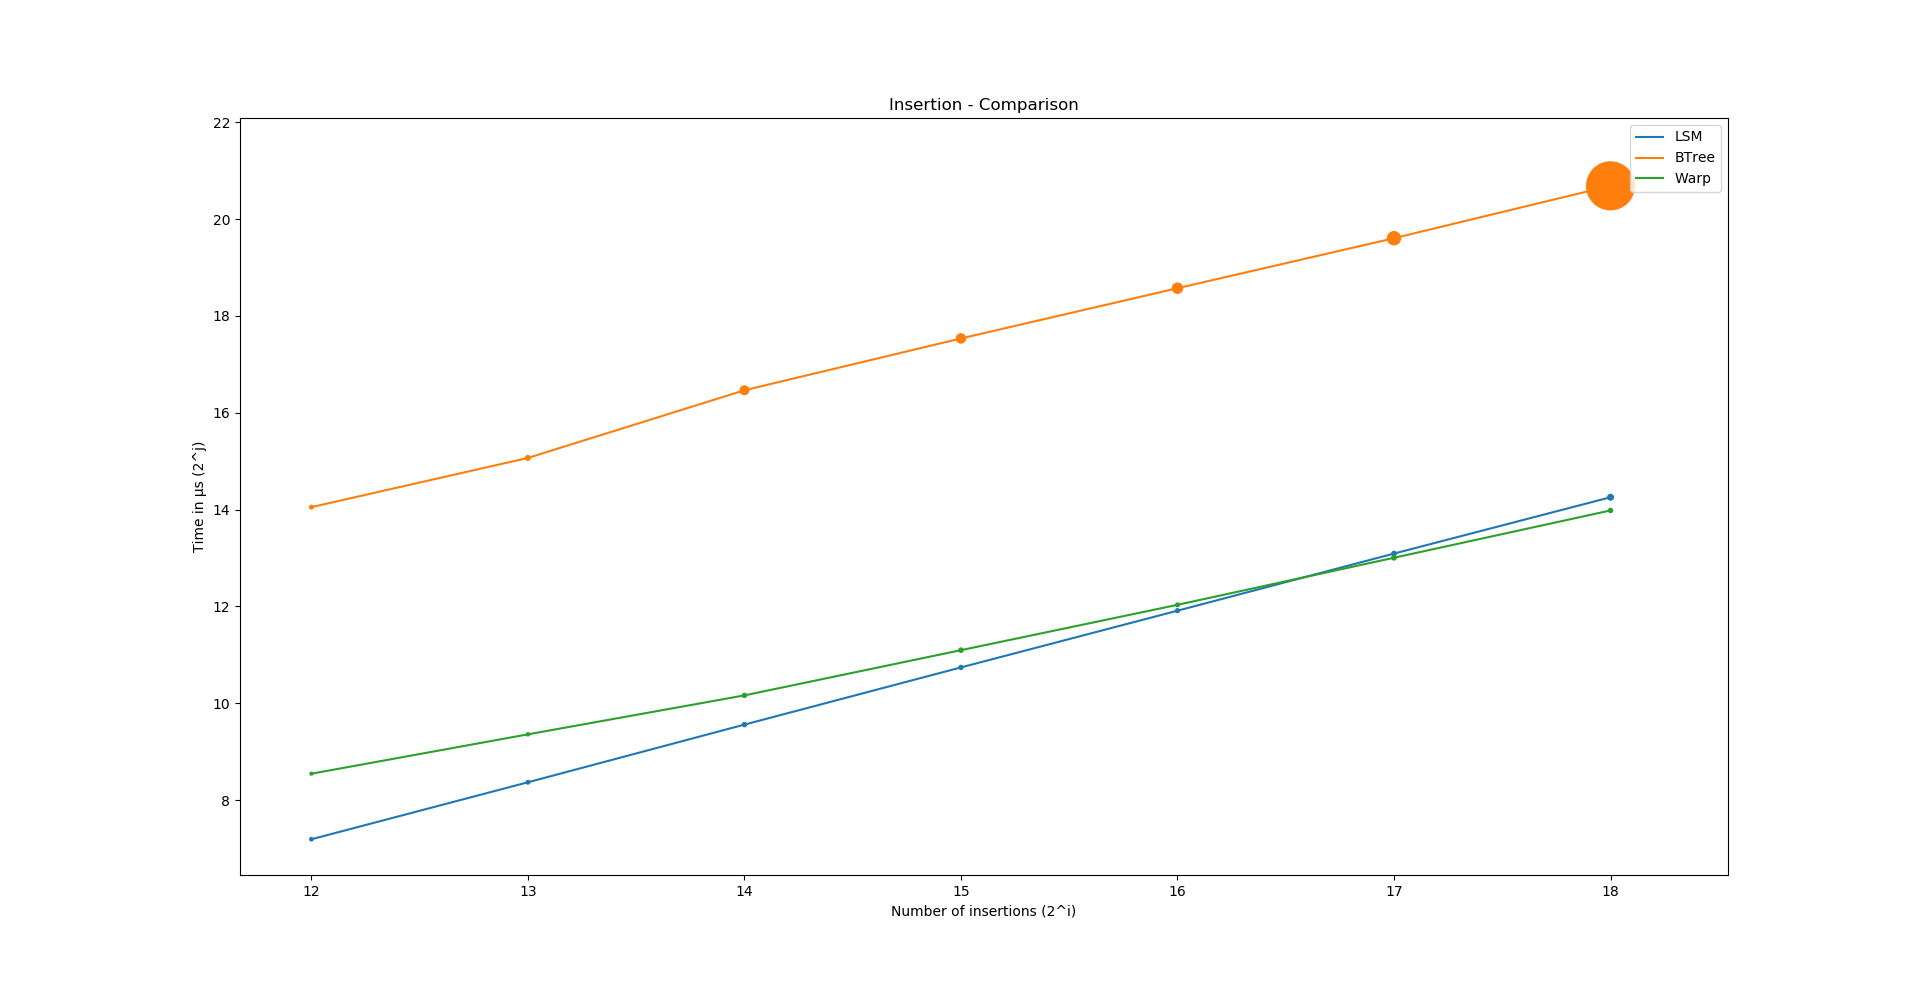
\includegraphics[width=\linewidth]{Chapters/ParallelXFastTries/Insertions.png} 
    \caption{32-bit key insertion}
\end{figure}

\begin{itemize}
    \item The standard deviation is a bit lower for X-fast tries\index{X-fast trie}. Indeed, it seems relatively clear that their variance is only dependent on the queries performed on the internal hash tables\index{Hash table}. But the load factor is relatively low, only 50\%, so it seems normal to have a narrow variance. On the contrary, we had already observed that the B-trees\index{B-tree} had a stronger tendency to have high variances related to the rebalancing necessary to maintain the structure in the tree. Finally, the LSM\index{LSM} have an associated variance relatively small in comparison to that of the B-trees\index{B-tree}, this is related to the cascading merge which must be carried out each time one passes to the next power of 2.
    \item The gain in concurrency that we have obtained by exploiting more warps for X-fast tries\index{X-fast trie} is very interesting. For both LSM\index{LSM} and X-fast tries\index{X-fast trie}, insertions are almost 100 times faster than for sequential B-trees\index{B-tree}.
    \item The LSM\index{LSM} offers lower starting constants but the coefficients of the larger orders seem larger. This does not seem so irrelevant since the merge operation is not totally without cost (the cost to sort the original buffer remains marginal~\cite{ashkiani2017parallel}). The LSM primitives are incredibly fast but the cascading mecanism remains significant on the performances.
    \item In this context, insertions in X-fast tries\index{X-fast trie} seem to be a good alternative to LSM\index{LSM}, following the batch size used of 512; and with greater flexibility, element-wise and not like in a bulk synchronous model. Note that the batch size presented in the original article was quite different, by a factor of more than 32 and that our implementation is not as optimal as their one.
\end{itemize}

We will continue with the two search operations:

We will start with thread-based queries:

\begin{figure}[!htb]
    \centering
    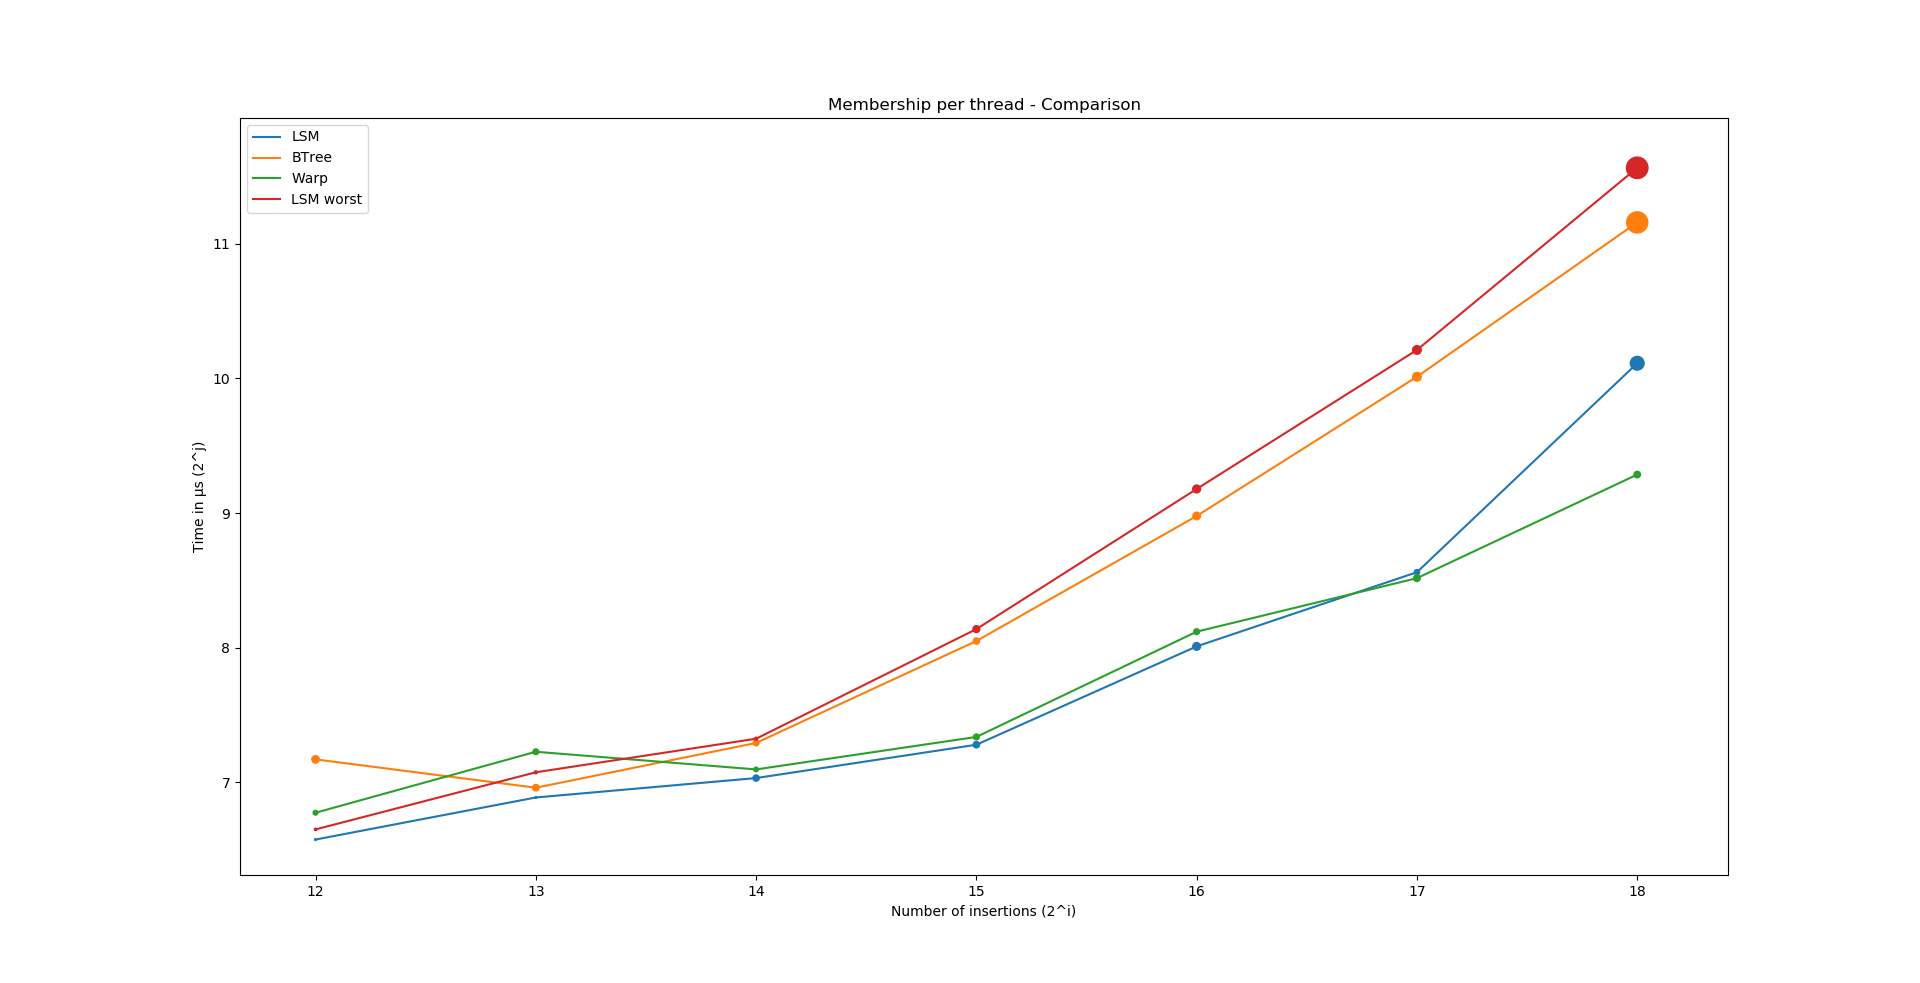
\includegraphics[width=0.85\linewidth]{Chapters/ParallelXFastTries/Membership_thread.png} 
    \caption{Thread-based searches}
\end{figure}

The results are somewhat astonishing:
\begin{itemize}
    \item Very logically, accessing X-fast tries\index{X-fast trie} elements is faster than for B-trees\index{B-tree}, since it consists of a simple search in a hash table\index{Hash table}, instead of running through an entire tree.
    \item But the difference between X-fast tries\index{X-fast trie} and LSM\index{LSM} is very surprising, they are really close. The main argument is related to the fact that the locality of the data is much stronger in the LSM\index{LSM}. The first pivots used during the dichotomous search, have strong chances to be kept in memory since they will be very often requested. We are also in the ideal situation for LSM where only one dichotomous search must be performed, since we have inserted a power of 2 elements ($b2^{k}$).
    \item When requests are made in the worst case for LSM, which corresponds to a number of insertions which is a power of 2 minus 1 ($b2^{k} - b$), the performances become comparable to that of a B-tree due to the potential $O(\log N)$ queries made. On average, the LSM remains better than the B-tree.
\end{itemize}

Now, the warp-based queries where the whole warp contributes to search one element:

\begin{figure}[!htb]
    \centering
    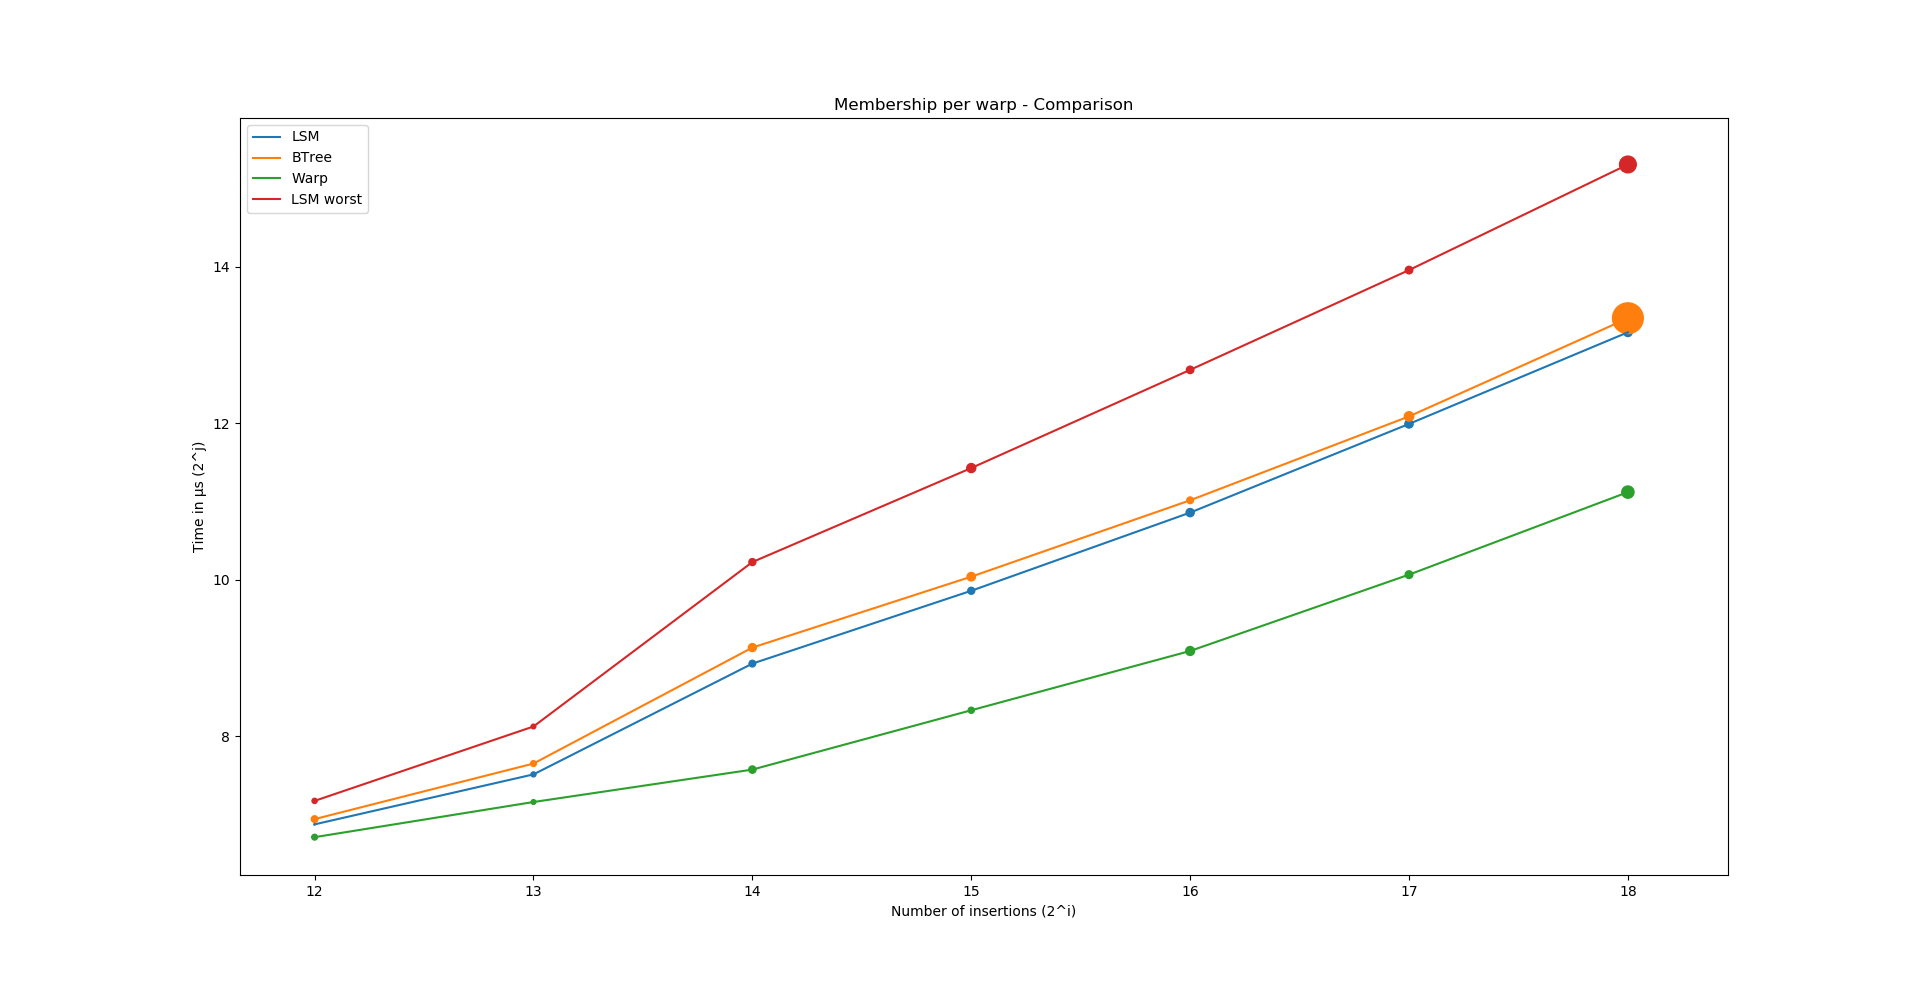
\includegraphics[width=0.85\linewidth]{Chapters/ParallelXFastTries/Membership_warp.png} 
    \caption{Warp-based searches}
\end{figure}

We observe similar phenomena:
\begin{itemize}
    \item The best case for LSM\index{LSM} is close to B-trees because dichotomous key searches no longer have to be performed. So all that remains is the cost of searching properly and loading the different blocks.
    \item X-fast tries\index{X-fast trie} retain their advantage thanks to the multiple probes performed at the same time in the leaf-level hash table\index{Hash table}.
\end{itemize}

\newpage

Finally, all we have left to observe are the predecessor's queries:

\begin{figure}[!htb]
    \centering
    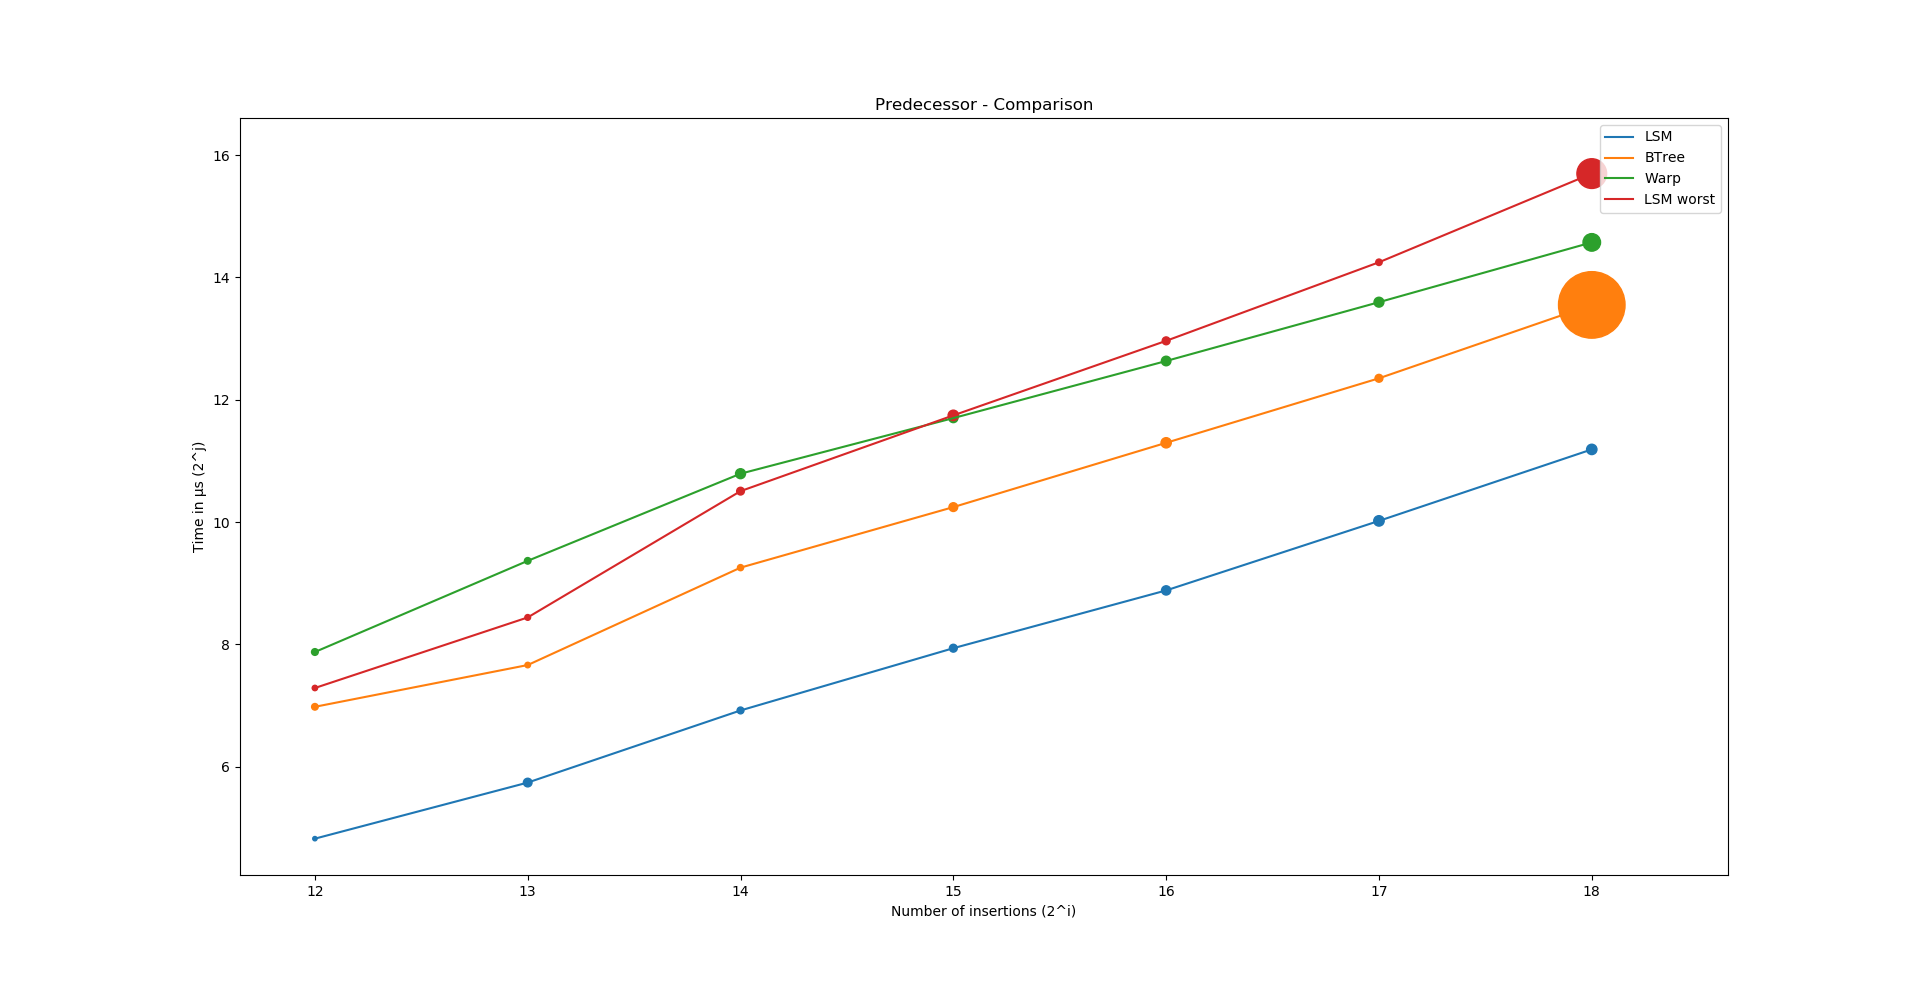
\includegraphics[width=\linewidth]{Chapters/ParallelXFastTries/Predecessor.png} 
    \caption{Warp-based predecessor queries}
\end{figure}

Some remarks can be made:
\begin{itemize}
    \item We notice the same phenomenon as in the sequential\index{Sequential} framework, X-fast tries\index{X-fast trie} are slower than B-trees\index{B-tree} because of their imposing number of memory requests.
    \item For the LSM\index{LSM}, the performance is roughly equivalent to the search operation, which is quite logical since both use lower bound algorithm.
    \item We precise that the predecessor search can be done by thread for LSM, whereas for X-fast tries, it can only be done by warp. So we simulated this operation by performing only one of the queries in the warp to make it comparable to other data structures.
    \item De facto, the time that would be taken to search for the predecessor per thread for LSM\index{LSM} would be even faster than pseudo warp-based, and a gain of a factor 8 would not seem excessive.
    \item Predecessor requests in X-fast tries are faster than those in a LSM in the worst case, but on average they are significantly slower.
\end{itemize}
